% !TEX root = ThesisGchatzi.tex

\chapter{State of the Art} \label{chap:related}
\graphicspath{{Papers/SIGSpatial2017/}{Papers/SIGSpatial2018/}{Papers/SpringerJournalOfBigData/}}

Time series management, mining and exploration has many applications across several industrial and scientific domains. Due to the complex nature of time series data, these tasks have attracted a lot of academic and research interest. As a result, there is a plethora of methods in the literature, that (i) apply various techniques to improve the management of large time series datasets, (ii) facilitate querying and extracting insightful information and (iii) ultimately enable the efficient exploration of such data. 

Furthermore, as the ubiquitous generation of information governs more and more aspects of human life, applying efficient analysis tasks on Big Data is a demanding task of increasing scientific and industrial importance. The simplicity along with the effectiveness of the $k$-Nearest Neighbors (kNN) algorithm, have motivated many research communities over the years with numerous applications and scientific approaches, which exploit or improve its potential on various data types, one of which being time series.

In the following sections, we outline related and state-of-the-art work on the above fields. More specifically, in Section~\ref{sec:ts_index_query_explore}, we discuss existing approaches for indexing, querying and visual exploration of time series and other types of data. In Section~\ref{sec:ts_search}, we outline related work on similarity search applied on time series data. Finally, Section~\ref{sec:knn_ml}, presents existing scalable approaches on $k$-Nearest Neighbors and dimensionality reduction.

\section{Time Series Indexing, Querying and Visual Exploration}
\label{sec:ts_index_query_explore}

\paragraph{Spatio-Textual Indices.} There is an increasing amount of spatio-textual objects, e.g., Points of Interest (PoI) with textual descriptions, geotagged tweets or posts in social media, etc. This has motivated research on hybrid spatial-keyword queries combining location-based predicates with keyword search. Main query types include the \emph{Boolean Range Query}, which retrieves all objects that contain a given set of keywords and are located within a specified spatial range; the \emph{Boolean $k$NN Query}, which returns the $k$ nearest objects to a specific location and contain the given keywords; and the \emph{Top-$k$ $k$NN Query}, which finds the top-$k$ objects according to an objective function that assigns hybrid scores to objects based on both their keyword similarity and spatial proximity to the query object \cite{chen2013pvldb}.

To evaluate such queries efficiently, the main idea is to construct hybrid index structures that simultaneously partition the data in both dimensions, spatial and textual. Essentially, this implies combining a spatial index structure (e.g., R-tree, Quadtree, Space-Filling Curve) with a textual index (e.g., inverted file, signature file). Depending on their form, the resulting variants can be characterized either as {\em spatial-first} or {\em textual-first} indices \cite{christoforaki2011cikm}. One of the most fundamental and characteristic ones is the IR-tree \cite{cong2009vldb,zhisheng2011tkde}, which extends the R-tree by augmenting the contents of each node with a pointer to an inverted file indexing terms and documents contained in its sub-tree. Several other hybrid spatio-textual indices extending the R-tree (or R$^*$-tree) have been proposed, such as the IR$^2$-tree \cite{defelipe2008icde}, the KR$^*$-Tree \cite{hariharan2007ssdbm}, SKI \cite{cary2010ssdbm} and S2I \cite{rocha2011ssd}, while methods based on space filling curves include SF2I \cite{chen2006sigmod} and SFC-QUAD \cite{christoforaki2011cikm}.

In this thesis, we introduce a new hybrid indexing method, the \btsr index, which is based on the R-tree \cite{Guttman1984} for the spatial indexing part. Recall that an R-tree organizes a hierarchy of nested $d$-dimensional rectangles. Each node corresponds to a disk page and represents the MBR of its children or, for leaf nodes, the MBR of its contained geometries. The number of entries per node (excluding the root) is between a lower bound $m$ and a maximum capacity $M$. Query execution in R-trees starts from the root. MBRs in any visited node are tested for intersection against a search region. Qualifying entries are recursively visited until the leaf level or until no further overlaps are found. Several paths may be probed, because multiple sibling entries could overlap with the search region.

All aforementioned approaches focus exclusively on combining spatial queries with keyword search. To the best of our knowledge, \btsr is the first one to address geolocated time series, combining spatial queries with similarity search for time series.

\paragraph{Time Series Indexing.} Earlier approaches towards indexing time series data were based on leveraging multi-resolution representations. For instance, the Discrete Wavelet Transform \cite{graps1995cse} is used in \cite{chan1999icde} to gradually reduce the dimensionality of time series data via the \emph{Haar wavelet} \cite{haar1910theorie} and generate an index using the coefficients of the transformed sequences. In \cite{popivanov2002icde}, it is further observed that, other than orthonormal wavelets, bi-orthonormal ones can also be used for efficient similarity search over wavelet-indexed time series data, demonstrating several such wavelets that outperform the Haar wavelet in terms of precision and performance. In addition, an alternative approach to the $k$-nearest neighbor search over time series data is introduced in \cite{kashyap2011kdd}. The proposed method accesses the coefficients of Haar-wavelet-transformed time series through a sequential scan over step-wise increasing resolutions.

State-of-the-art approaches for time series indexing comprise methods based on the {\em Symbolic Aggregate Approximation} (SAX) representation \cite{jessica2007dmkd}. It is a multi-resolution representation of a time series introduced in \cite{shieh2008kdd}. It can be derived from its {\em Piecewise Aggregate Approximation} (PAA) \cite{keogh2001paa,faloutsos2000vldb} by quantizing the PAA segments on the $v$-axis. As exemplified in Figure~\ref{subfig:isax_representation}, a time series $T_2$ is transformed to a PAA representation of $w$=3 words with real-valued coefficients (the horizontal red bars). To get a $SAX$ representation for a time series, these coefficients are discretized along the $v$-axis using {\em breakpoints} (shown with dashed lines) assuming a $\mathcal{N}(0,1)$ Gaussian distribution that enables generation of equi-probable symbols for a given cardinality ($b=4$ symbols are used in this example). Interestingly, by using bitwise representations for these symbols, coarser $SAX$ values can be obtained from more refined ones by simply ignoring trailing bits. Importantly, the Euclidean distance between $SAX$ representations of two time series is guaranteed to be a {\em lower bound} with respect to the Euclidean distance over the original time series. Formally, for two time series $T, T'$ of equal length $n$ using their respective $SAX$ words $T_w, T'_w$ of size $w$, it holds that:

\begin{equation} \label{eq:dist_sax}
dist_{SAX}(T_w, T'_w) =\sqrt{\frac{n}{w}} \sqrt{\sum_{j=1}^{w} d^2(t_j, t'_j) }  \leq {\sqrt{\displaystyle \sum_{i=1}^{n}(T.v_i - T'.v_i)^2}}
\end{equation}

\noindent where $d(t_j, t'_j)$ is the distance between symbols at the $j$-th position of each $SAX$ word. Comparing \isax words of different cardinality is possible by promoting the \isax representation of lower cardinality to that of the larger, as the lower bound in Eq.~\ref{eq:dist_sax} still holds.

\begin{figure}[!t]
 \centering
 \subfloat[SAX of a time series]{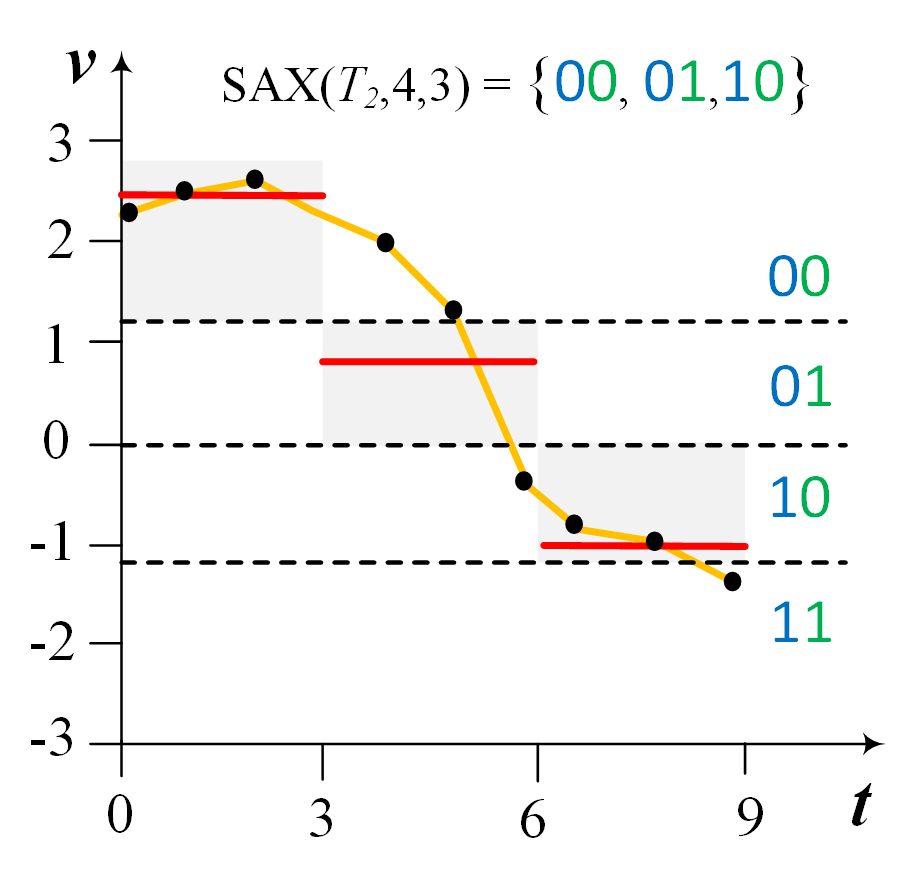
\includegraphics[width=0.4\textwidth]{figures/sax2.png}\label{subfig:isax_representation}}
 \subfloat[MBTS for two sets of time series]{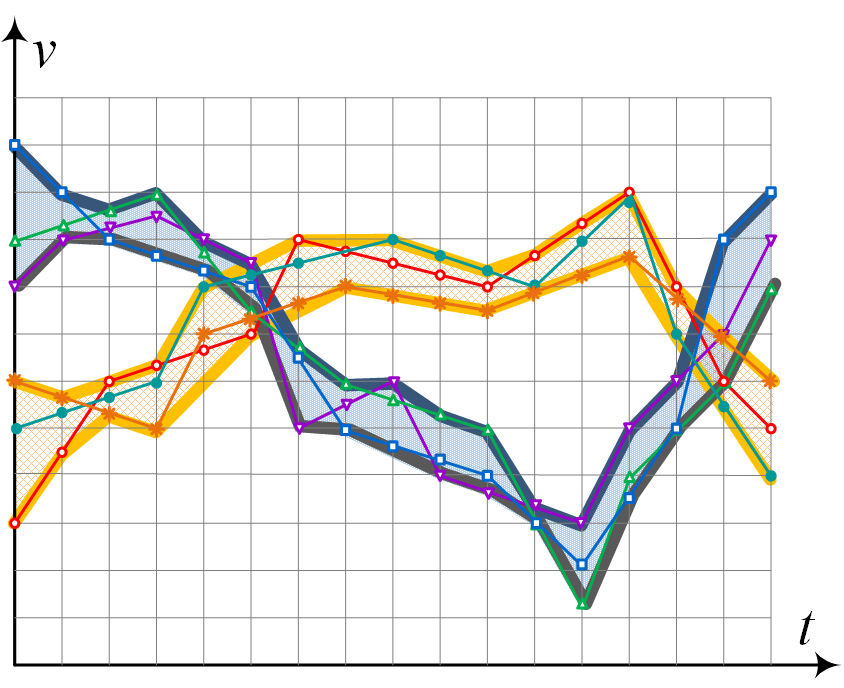
\includegraphics[width=0.5\textwidth]{figures/bounds_ctsr.png}\label{fig:example_bundle}}
\caption{SAX and MBTS representations over time series.}
\label{fig:isax_example}
\end{figure}

The first attempt to leverage the potential of the SAX representation was presented in \cite{shieh2008kdd}, introducing the indexable Symbolic Aggregate Approximation ($i$SAX), capable of a multi-resolution representation for time series. Considering a set of time series, an \isax index \cite{shieh2008kdd} can be built as illustrated in Figure~\ref{fig:isaxtree}. The root node captures the complete \isax space. It does not contain any SAX words, it only points to its children nodes (in the worst case, their number is $2w$). Each leaf has a pointer to a disk file containing the raw time series that it represents. The leaf itself also stores the \isax word of highest cardinality among these time series. An internal node designates a split in SAX space and is created when the number of time series contained by a leaf node exceeds a fixed capacity $M$. This split is binary and is made at a given position $j=1..w$ of the SAX word using a round-robin policy, so it always yields two children that differ on their $j$-th symbol while replicating the rest from their parent node. In essence, the SAX space represented by every node fully contains the union of the SAX spaces of its subtree.

\isax can answer {\em similarity queries}, and thus can be also used in $k$-nearest neighbor search \cite{shieh2008kdd}. Searching for time series similar to a given query time series simply traverses the \isax tree, looking for a leaf node having the same \isax word as the query. The respective raw times series are fetched from disk and a sequential scan identifies those matching with $q$. The iSAX index was further extended to $i$SAX 2.0 in \cite{camerra2010icdm} by enabling bulk loading of time series data. Its next version is the $i$SAX2+ index \cite{camerra2014kais}, which handles better the expensive I/O operations caused by the aggressive node splitting while building the index. Finally, the ADS+ index \cite{zoumpatianos2014sigmod} is another extension of $i$SAX, which attempts to overcome the still significantly expensive index build time by adaptively building the index while processing the workload of queries issued by the user. A comprehensive overview and comparison of the time series indexing approaches based on the SAX representation is presented in \cite{palpanas2016bigsm}.

\begin{figure}[!t]
 \centering
 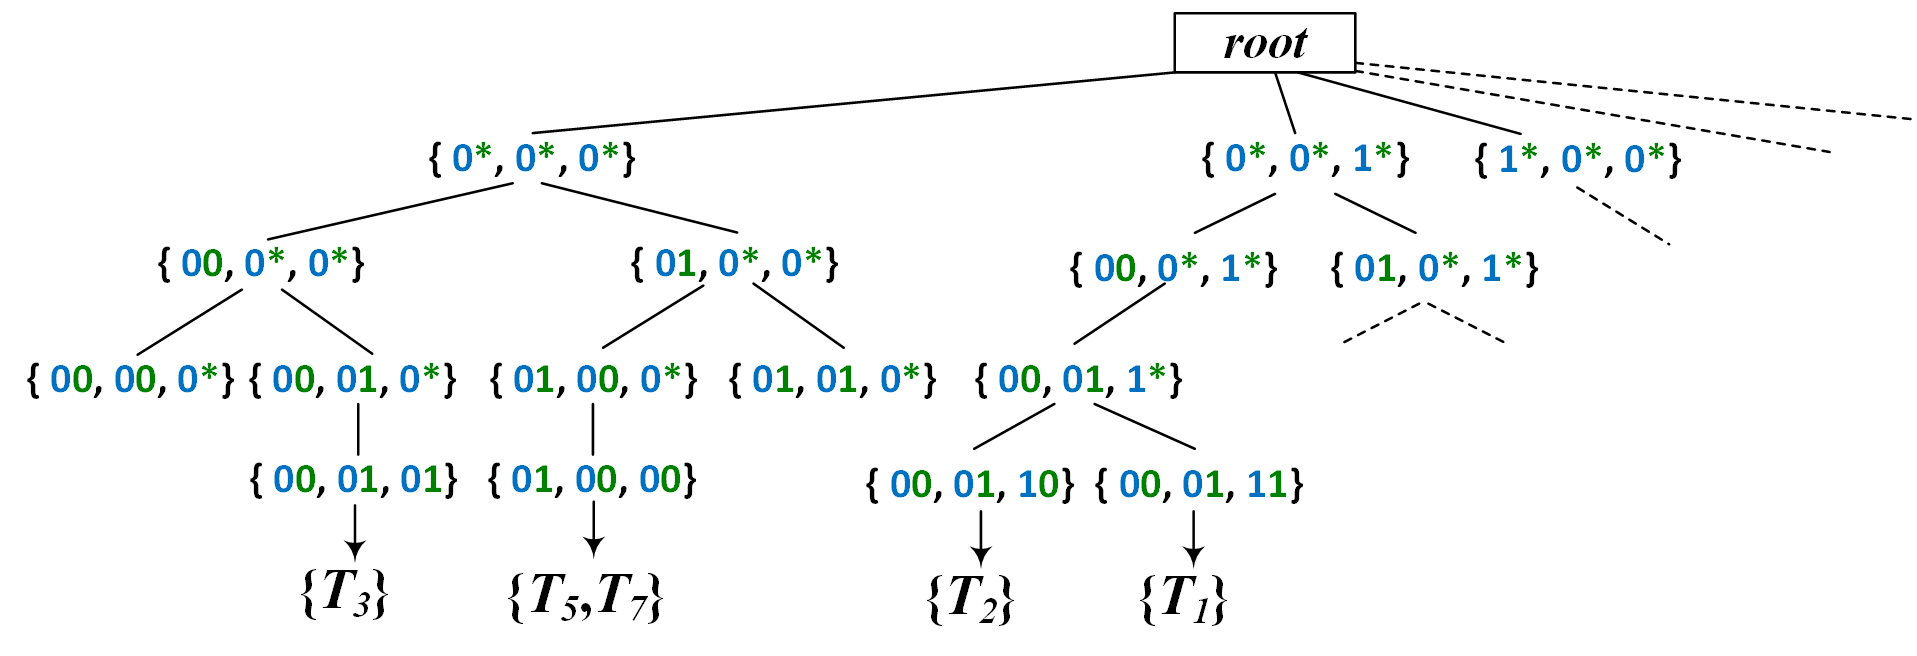
\includegraphics[width=\textwidth]{figures/isax_tree2.png}
 \caption{\isax index over time series.}
 \label{fig:isaxtree}
\end{figure}

Contrary to \btsr, none of the above approaches supports geolocated time series, and thus cannot efficiently process hybrid queries combining time series similarity with spatial proximity.

\paragraph{Spatial Join Queries} With respect to {\em spatial join queries}, several methods have been proposed, often based on the R-tree family of indices \cite{Guttman1984, Beckmann1990}. In particular, the spatial join algorithms over R$^*$-trees introduced in \cite{DBLP:conf/sigmod/BrinkhoffKS93} can minimize the CPU and I/O cost in searching. {\em Multiway} spatial joins \cite{papadias1999processing} generalize search over more than two R-trees. Top-$k$ spatial distance joins~\cite{qi2013efficient} employ R-tree-based spatial joins in data blocks ordered by an objective score to retrieve $k$ pairs of objects with highest score. However, all such algorithms are applied against spatial information only. Based on a similar observation for answering a variety of queries over geolocated time series, in \cite{chatzig17btsr} we proposed the \btsr, a hybrid index based on the R-tree, but having nodes that also store bounds over the time series information in their underlying subtree. This index offers increased pruning capabilities for queries involving both time series similarity and spatial proximity. However, handling hybrid similarity joins is not addressed in \cite{chatzig17btsr}; we develop such a method next in this thesis.

Our work on geolocated time series similarity join queries using the \btsr index is reminiscent of related approaches in {\em spatio-textual search}. Spatio-textual joins identify objects that are both spatially and textually close. In particular, the algorithm proposed in \cite{Bouros:2012:SSJ:2428536.2428537} uses a spatial partitioning in conjunction with spatial joins over R-trees in order to batch process such queries. MapReduce-based methods in \cite{Zhang:2014:ESS:2682647.2682773} resolve spatio-textual joins on spatially partitioned data. However, it should be stressed that time series information is quite distinct from documents or keywords used in those works and certainly requires a totally different processing paradigm. To the best of our knowledge, ours is the first approach for processing similarity joins on geolocated time series data.

\paragraph{Visual Exploration of Time Series.} Numerous approaches attempt to leverage the potential of summarizing or aggregating the information of large time series data to facilitate visual exploration and knowledge extraction. An early approach is~\cite{mintz1997tracking}, where the authors use tile maps and box plots to discover ten-year trends in air pollution data. In \cite{keim1995recursive}, the authors introduce a pixel-oriented visualization to detect recursive patterns, where each data value is represented by one pixel. The authors demonstrate the potential of their method using a stock market dataset. An extension of this work is presented in~\cite{lammarsch2009hierarchical}, where several time granularities are combined in a single visualization to enhance the knowledge extraction potential of recursive patterns. 

Of particular interest are visualization approaches that attempt to leverage the potential of declarative SQL-like languages and DBMSs to enable exploratory queries. Such an approach is suggested in M4~\cite{jugel2014m4}, where the authors introduce an aggregation-based dimensionality reduction scheme for visualizing horizontally large time series using line charts. Their approach operates on top of an RDBMS and supports various SQL queries that select and visualize particular parts of time series. ForeCache \cite{battle2016sigmod} leverages two prefetching mechanisms to facilitate exploration of large geospatial, multidimensional and time series data stored in a DBMS. By predicting the user's behavior, it fetches the necessary data as the user interacts with the application. Another declarative language-based visualization is suggested in \cite{wu2014vldb}, where relational algebra queries are used to represent the visualization, leveraging the potential of traditional and visualization-specific optimizations. In contrast, a recent tutorial \cite{mottin2017vldb} advocates the use of example-based methods in exploration of large relational, textual, and graph datasets. Such a {\em query-by-example} approach has been applied in \cite{eravci2013vldb} so as to explore relevance feedback for retrieval from time series databases. Instead of returning the top matching time series, this technique incorporates diversity into the results, which are presented to the user for feedback and refined in several rounds.

RINSE \cite{zoumpatianos2015vldb} is a Recursive Interactive Series Explorer specifically designed for exploration of data series. Built on top of ADS+ \cite{zoumpatianos2014sigmod}, a special adaptive index structure for data series, it can progressively build parts of the index on demand at query time, concerning only those chunks of the data involved in users' queries. In terms of visualization, users can get those series qualifying to range or nearest-neighbor queries interactively drawn on screen, as well as monitor various statistics regarding the index footprint (e.g., RAM and disk usage) as it gets updated. In contrast, ATLAS \cite{chan2008vast} is a visual analytics tool specifically geared towards interactivity when ad hoc filters, arbitrary aggregations, and trend exploration are applied against massive time series data. This client-server architecture employs a column store as its backend equipped with indexing, and preemptively caches data that may be required in queries so as to reduce latency when {\em panning}, {\em scrolling}, and {\em zooming} over time series. Recently, the ONEX paradigm \cite{neamtu2016vldb} concerns online exploration of time series. It first constructs compact similarity groups over time series for specific lengths based on Euclidean distance, and then can efficiently support exploration of these groups with the Dynamic Time-Warping (DTW) method over their representatives of different lengths and alignments. {\em Smoothing} can be applied to streaming time series to remove noise in visualizations while preserving large-scale deviations \cite{rong2017vldb}. To highlight important phenomena without harming representation quality from oversmoothing, this approach introduces quantitative metrics involving variance of first differences and kurtosis to automatically calibrate smoothing parameters.

The ability to zoom in to specific parts of interest of a large time series can significantly enhance the exploratory potential of a visualization. Stack zooming~\cite{javed2010stack} provides such a functionality, by building hierarchies of line chart visualizations for user-defined intervals on large time series data. Each selected interval is zoomed and stacked beneath the initial time series. A similar approach is KronoMiner~\cite{zhao2011kronominer}, which employs a radial-based visualization to enable zooming functionality for specific time intervals. The interface is visually refined through an iterative design procedure involving expert user feedback. ChronoLenses \cite{zhao2011exploratory} introduces a domain-independent visualization that offers the ability to perform on-the-fly transformations (e.g., Fourier transform, auto-correlation) of the selected interval using {\em lenses}.

Zooming in regions of interest in time series can be performed via {\em timeboxes}, which essentially consist of rectangular regions on the time series domain thus specifying intervals in both the time and value axis. The procedure retrieves the time series whose values in the given region are fully contained in the rectangle. Hochheister et al. introduced timeboxes~\cite{hochheiser2004dynamic} along with {\em TimeSearcher}, an application for visual exploration of time series datasets that implements timebox queries. The user is able to draw rectangles on the time series domain and the results are separately displayed on-screen. Keogh et al.~\cite{keogh2002augmented} extended the timeboxes, introducing the {\em Variable Time Timeboxes}, which allowed a degree of uncertainty in the time axis. Later versions of TimeSearcher (such as ~\cite{aris2005representing}) provided enhanced functionality, allowing the visual exploration of longer time series ($>$10,000 time points) and offering forecasting functionality.

None of the aforementioned methods and systems provides map-based visual exploration of {\em geolocated} time series. In this thesis, we introduce a summary construction method for geolocated time series, that utilizes our spatial-first \btsr index, to enable spatial-domain map-based exploratory visualizations. Further, we introduce a {\em time series-first} hybrid index to facilitate timebox search on both horizontally and vertically large time series datasets. We enable efficient exploration on geolocated time series datasets, by timely executing user-defined timebox search, enabling the exploration also in the time series domain.

\section{Time Series Similarity Search}
\label{sec:ts_search}

\paragraph{Correlated Time Series.} Identifying similar subsequences between time series also indicates some {\em correlation} between them. Several approaches compute pairwise statistics (e.g., Pearson correlation, beta values) especially in streaming time series \cite{zhu2002statstream,cole2005fast,papadimitriou2006local}. There are also works concerning {\em co-evolving} time series data, either towards detecting and correcting missing values \cite{yongjie2015fast} or mining typical patterns and points of variation to achieve a meaningful segmentation of large time series \cite{matsubara2014autoplait}. However, none of these approaches is applicable to our setting, where we require similarity in the time series values. 

\paragraph{Time series clustering.} Our work also relates to {\em clustering of time series}, where methods perform either partitioning or density-based clustering. In the former class, algorithms typically partition the time series into $k$ clusters. Similarly to iterative refinement employed in $k$-means, the $k$-Shape partitioning algorithm~\cite{Paparrizos:2015:KEA:2723372.2737793,Paparrizos:2017:FAT:3086510.3044711} aims to preserve the shapes of time series assigned to each cluster by considering the shape-based distance, a normalized version of the cross-correlation measure between time series. In contrast, density-based clustering methods are able to identify clusters of time series with arbitrary shapes. YADING~\cite{Ding:2015:YFC:2735479.2735481} is a highly efficient and accurate such algorithm, which consists of three steps: it first samples the input time series also employing PAA (Piecewise Aggregate Approximation) to reduce the dimensionality, then applies multi-density clustering over the samples, and finally assigns the rest of the input to the identified clusters. However, clustering methods consider time series in their entirety and not matching subsequences as we consider in this thesis.

\paragraph{Subsequence matching.} The problem of {\em subsequence matching} over time series is to identify matches of a (relatively short) query subsequence across one or more (relatively long) time series. The UCR suite \cite{rakthanmanon2012searching} offers a framework comprising various optimizations regarding subsequence similarity search. Matrix Profile~\cite{yeh2016matrix} includes methods for detecting, for each subsequence of a time series, its \textit{nearest neighbor} subsequence, by keeping track of Euclidean distances among candidate pairs. Applying such approaches in our setting is not straightforward. First, they involve Euclidean or DTW distances, which are different from our definition of local similarity score (see Section~\ref{subsec:local_sim_search_problem}, hence the pruning heuristics do not hold in our case. Second, they do not consider geolocated time series, thus spatial filtering has to be carried out independently, which reduces pruning opportunities.

\paragraph{Similarity Search.} Similarity search over time series has attracted a lot of research interest~\cite{DBLP:journals/pvldb/EchihabiZPB18}. One well-studied family of approaches includes wavelet-based methods~\cite{chan1999icde}, which rely on \emph{Discrete Wavelet Transform}~\cite{graps1995cse} to reduce the dimensionality of time series and generate an index using the coefficients of the transformed sequences. The \emph{Symbolic Aggregate Approximation} (SAX) representation~\cite{jessica2007dmkd} has led to the design of a series of indices, including $i$SAX~\cite{shieh2008kdd}, $i$SAX 2.0~\cite{camerra2010icdm}, $i$SAX2+~\cite{camerra2014kais}, ADS+~\cite{zoumpatianos2014sigmod}, Coconut~\cite{DBLP:journals/pvldb/KondylakisDZP18}, DPiSAX~\cite{dpisaxjournal}, and ParIS~\cite{DBLP:conf/bigdataconf/PengFP18}. However, these indices support similarity search over complete time series, i.e. whole-matching. Recently, the \textit{ULISSE} index was proposed~\cite{linardi2018scalable}, which is the first index that can answer similarity search queries of variable length. 

Moreover, many approaches have been proposed for subsequence matching. In this problem, a query subsequence is provided and the goal is to identify matches of this subsequence across one or more time series, typically of large length. The \textit{UCR suite} \cite{rakthanmanon2012searching} offers a framework comprising four different optimizations regarding subsequence similarity search. In computing \textit{full-similarity-joins} over large collections of time series, i.e., to detect for each possible subsequence its \textit{nearest neighbor}, the \textit{matrix profile}~\cite{yeh2016matrix} keeps track of Euclidean distances among each pair within a \textit{similarity join set} (i.e., a set containing pairs of each subsequence with its nearest neighbor).

The problem of pair and bundle discovery that we address in this thesis differs from the above settings. Instead of identifying matches of a query subsequence against one, or more time series, we are interested in discovering locally similar pairs and bundles of time-aligned subsequences within a given collection of time series.

\paragraph{Discovery of Movement Patterns in Trajectories.} Finally, our work on pair and bundle discovery also relates to approaches for discovering clusters of moving objects, in particular a type of movement patterns that is referred to as {\em flocks}~\cite{gudmundsson2006computing}. A flock is a group of at least $m$ objects moving together within a circular disk of diameter $\epsilon$ for at least $\delta$ consecutive timestamps. Finding an exact flock is NP-hard, hence this work suggests an \textit{approximate} solution to find the \textit{maximal} flock from a set of trajectories using computational geometry concepts. In \cite{benkert2008reporting}, another \textit{approximate} solution for detecting all flocks is based on a skip-quadtree that indexes sub-trajectories. Flock discovery over {\em streaming} positions from moving objects was addressed in \cite{vieira2009line}. This \textit{exact} solution discovers flock disks that cover a set of points at each timestamp. Their flock discovery algorithm finds candidate flocks per timestamp and joins them with the candidate ones from the previous timestamps, reporting a flock as a result when it exceeds the time constraint $\delta$. An improvement over this technique was presented in \cite{tanaka2015efficient}, using a \textit{plane sweeping} technique to accelerate detection of object candidates per flock at each timestamp, while an inverted index speeds up comparisons between candidate disks across time. In our setting, detection of bundles is similar to flocks, thus for our baseline method we adapt the algorithm from \cite{vieira2009line}.

\section{Scalable \texorpdfstring{$k$}--Nearest Neighbors and Machine Learning}
\label{sec:knn_ml}

\paragraph{\texorpdfstring{$k$}--Nearest Neighbors.} Several works in the literature have reported the superiority of $k$-nearest neighbors on machine learning tasks over similar approaches, both in terms of processing time, as well as in terms of accuracy~\cite{amancio2014systematic, yang1999evaluation, colas2009data}. There are numerous approaches that exploit its potential. Zhang et al.~\cite{linkg2005multi} introduced a multi-label classification method based on $k$NN which uses a \textit{Maximum a Posteriori} (MAP) principle to predict the class of an new element. Oswald et al.~\cite{oswald2001traffic} used an approximate $k$NN-based regression approach in order to forecast traffic flow. Wei and Keogh~\cite{wei2006semi} presented that an $1$NN classifier outperforms other similar methods in terms of error rate, when applied on time-series data. Xu~\cite{Xu2011mwk} introduced a multi-label weighted $k$NN classifier, where the weights for each class are computed via mathematical optimization, using Least Squared Errors (LSE). Gou et al.~\cite{Gou2011jcp} presented a weighted voting scheme for such classifiers, where the distance between an element and its nearest neighbors determines the weight of each neighbor's vote. The query element is classified to the most weighted class. Our FML-$k$NN framework extends this functionality by also calculating the probability of each element belonging to each class. Also, by employing a $k$-nearest neighbors joins approach, we allow for simultaneous classification or regression on datasets of really high volume, addressing the challenges that arise when processing Big Data in a distributed environment.

\paragraph{Dimensionality Reduction and Space Filling Curves.} Similarly to many data analysis and management tasks, $k$NN joins suffer from the \textit{curse of dimensionality}~\cite{berchtold1998his}. Liao et al.~\cite{liao2001SFC} stated that as the number of dimensions increases, such techniques need an exponentially larger amount of CPU time. Consequently, executing a $k$NN joins method on Big Data requires prohibitively long-lasting operations. To overcome this issue, \textit{dimensionality reduction} can be applied on the datasets by indexing their elements via a \textit{Space Filling Curve} (SFC)~\cite{sagan2012space}. This approach reduces data dimensionality to one dimension, which allows for a significantly faster execution of an approximate nearest neighbor search, based on the indexed elements. The most widely used SFCs are the \textit{$z$-order}, \textit{Gray-code} and \textit{Hilbert}, among which Mokbel et al.~\cite{mokbel2002pms} concluded that Hilbert is the most ``fair'', due to the fact that two consecutive points in the curve are always nearest neighbors. Yao et al.~\cite{yao2010knn} used the $z$-order curve to significantly boost the query performance over huge amounts of data. Lawder et al.~\cite{lawder2001qmd} efficiently executed range queries in data indexed by the Hilbert curve, while Faloutsos~\cite{faloutsos1986mhu} presented a mathematical model for indexing the multi-attribute records of a data collection, using Gray-codes instead of binary values. Similarly, Chatzigeorgakidis et al.~\cite{chatzigeorgakidis2015mapreduce} and Zhang et al.~\cite{zhang2012epk} exploit the $z$-order curve in order to perform $k$NN joins on a distributed environment. To support selection variety, our framework can operate by tuning and using the most preferable among these SFC methods, as space traversal quality and computation performance may differ according to the data context. Figure~\ref{figure1} shows an example of the recursive way the three SFCs scan the elements in a two-dimensional space.

\begin{figure}[!t]
	\centering
	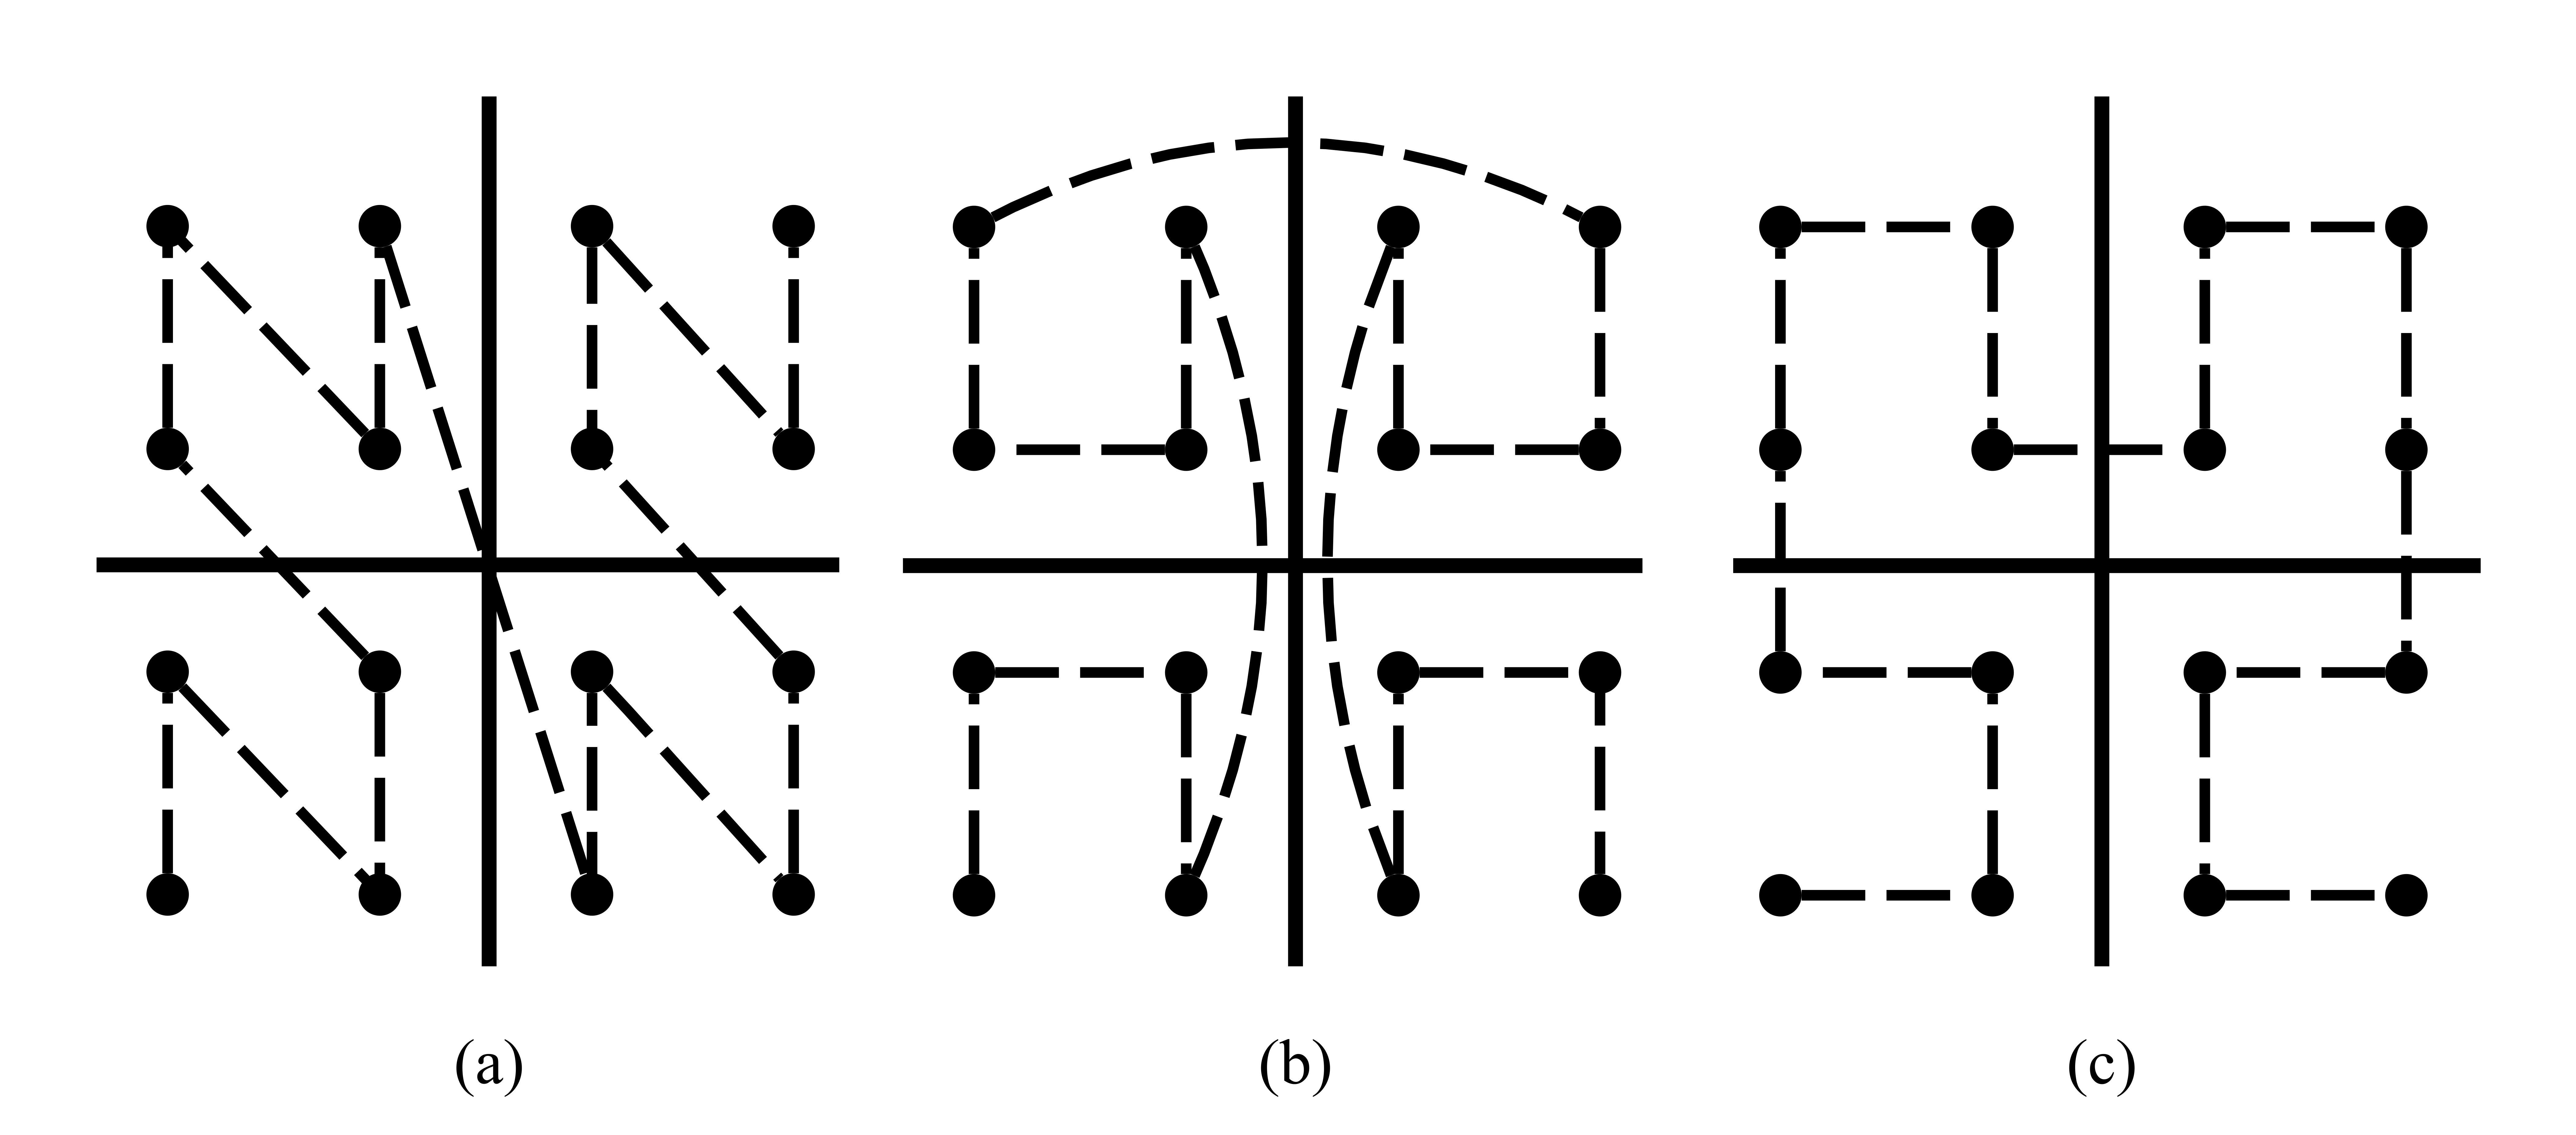
\includegraphics[width=0.75\textwidth]{figures/figure1.png}
	\caption{The three Space Filling Curves: (a) $z$-order curve, (b) Gray-code curve (c) Hilbert curve.}
	\label{figure1}
\end{figure}

\paragraph{\texorpdfstring{$k$}--Nearest Neighbors on Distributed Environments} The increasing scientific interest in the Big Data area has introduced modern distributed implementations of famous algorithms. More particularly, several approaches of MapReduce-based $k$NN joins algorithms have been proposed. Song et al.~\cite{song2015hal} present a review of the most efficient among them, denoting that all share the same three processing stages, i.e., (i) \textit{data pre-processing}, (ii) \textit{data partitioning and organization}, and (iii) \textit{$k$NN computation} stage. They conclude that the SFC-based H-$zk$NNJ~\cite{zhang2012epk} algorithm, outperforms in terms of completion time other similar methods like \textit{RankReduce}~\cite{stupar2010rankreduce}, which uses \textit{Locality Sensitive Hashing} (LSH)~\cite{indyk1998ann}. In~\cite{chatzigeorgakidis2015mapreduce}, we extended the functionality of H-$zk$NNJ~\cite{zhang2012epk}, by delivering the F-$zk$NN probabilistic classifier, which performs classification on the results of a $k$NN joins query. The F-$zk$NN probabilistic classifier is based on the MapReduce programming model and executed in a single distributed session. However, the datasets need to be propagated between the first two execution stages using local caches, which results in increased communication costs. Our approach optimizes F-$zk$NN by avoiding this costly propagation using Flink's broadcast sets and augments its functionality by incorporating an additional regression analysis operation. Both the probabilistic classifier and the regressor are included in our framework and are experimentally applied on water consumption related Big Data analysis tasks.

\paragraph{\texorpdfstring{$k$}--Nearest Neighbors in Resources Consumption Domain} Similar approaches which apply machine learning methods on resource consumption data (e.g., energy, water) but still not from a Big Data perspective, include the work of Chen et al.~\cite{chen2011aab} who used a $k$NN classification method and labeled water data to identify water usage. Naphade et al.~\cite{swp2011} and Silipo and Winters~\cite{bdse2013} focused on identifying water and energy consumption patterns, providing analytics and predicting future consumptions but in high granularity levels and in small scale. Schwarz et al.~\cite{schwarz2012lpss} used $k$NN for classification and short-term prediction in energy consumption by using smart meter data, however, they focused on in-memory and non-distributed approaches, thus, limiting the applicability on larger datasets. Our approach in the consumption domain partially relates to the work of Kermany et al.~\cite{Kermany2013aam}, where the $k$NN algorithm was applied for classification on water consumption data, in order to detect irregular consumer behavior. We take a step forward by applying our algorithm on two real-world case studies, delivering predictive analytics for water consumption in a Big Data scale.